\section{Results}
\label{sec:results}
\paragraph{Performance metrics}
\Cref{tab:scores-dialog} and \Cref{tab:scores-narration} show
the performance of several model configurations on the retrieval and
triplet tasks on the dialog and narration datasets respectively.

In the case of the narration data this scores is not confounded by
speaker-based clues, which is an indication that the model possibly
learned to detect some aspects of utterance meaning. We investigate
this hypothesis further using multiple representational similarity
analysis.
 

 \begin{table}
   \centering
   \begin{tabular}{rlrr}
\toprule
 ID & Pretraining &  Recall@10 &  Triplet Acc \\
\midrule
 43 &          AV &      0.193 &        0.814 \\
 44 &           V &      0.084 &        0.728 \\
 45 &        None &      0.034 &        0.597 \\
\bottomrule
\end{tabular}

   \caption{Retrieval and triplet scores on dialog validation data.}
   \label{tab:scores-dialog}
 \end{table}

\begin{table}
   \centering
   \begin{tabular}{rlrr}
\toprule
 ID & Pretraining &  Recall@10 &  Triplet Acc \\
\midrule
 43 &          AV &      0.239 &        0.866 \\
 44 &           V &      0.166 &        0.822 \\
 45 &        None &      0.087 &        0.741 \\
\bottomrule
\end{tabular}

   \caption{Retrieval and triplet scores on narration validation data.}
   \label{tab:scores-narration}
 \end{table}
 
\paragraph{Targeted Triplets}
\todo{add average targeted triplets result to general performance metrics table?}

We report results for the best performing model according to the performance metrics (ID 48, audio and video pretraining). The average targeted triplets accuracy is 0.726 . \Cref{fig:accuracy_targeted_triplets_nouns} and \Cref{fig:accuracy_targeted_triplets_verbs} show per-word accuracy for nouns and verbs, respectively. The vertical bars indicate the standard deviation as estimated using bootstrapping tests.


\begin{figure}
  \centering
  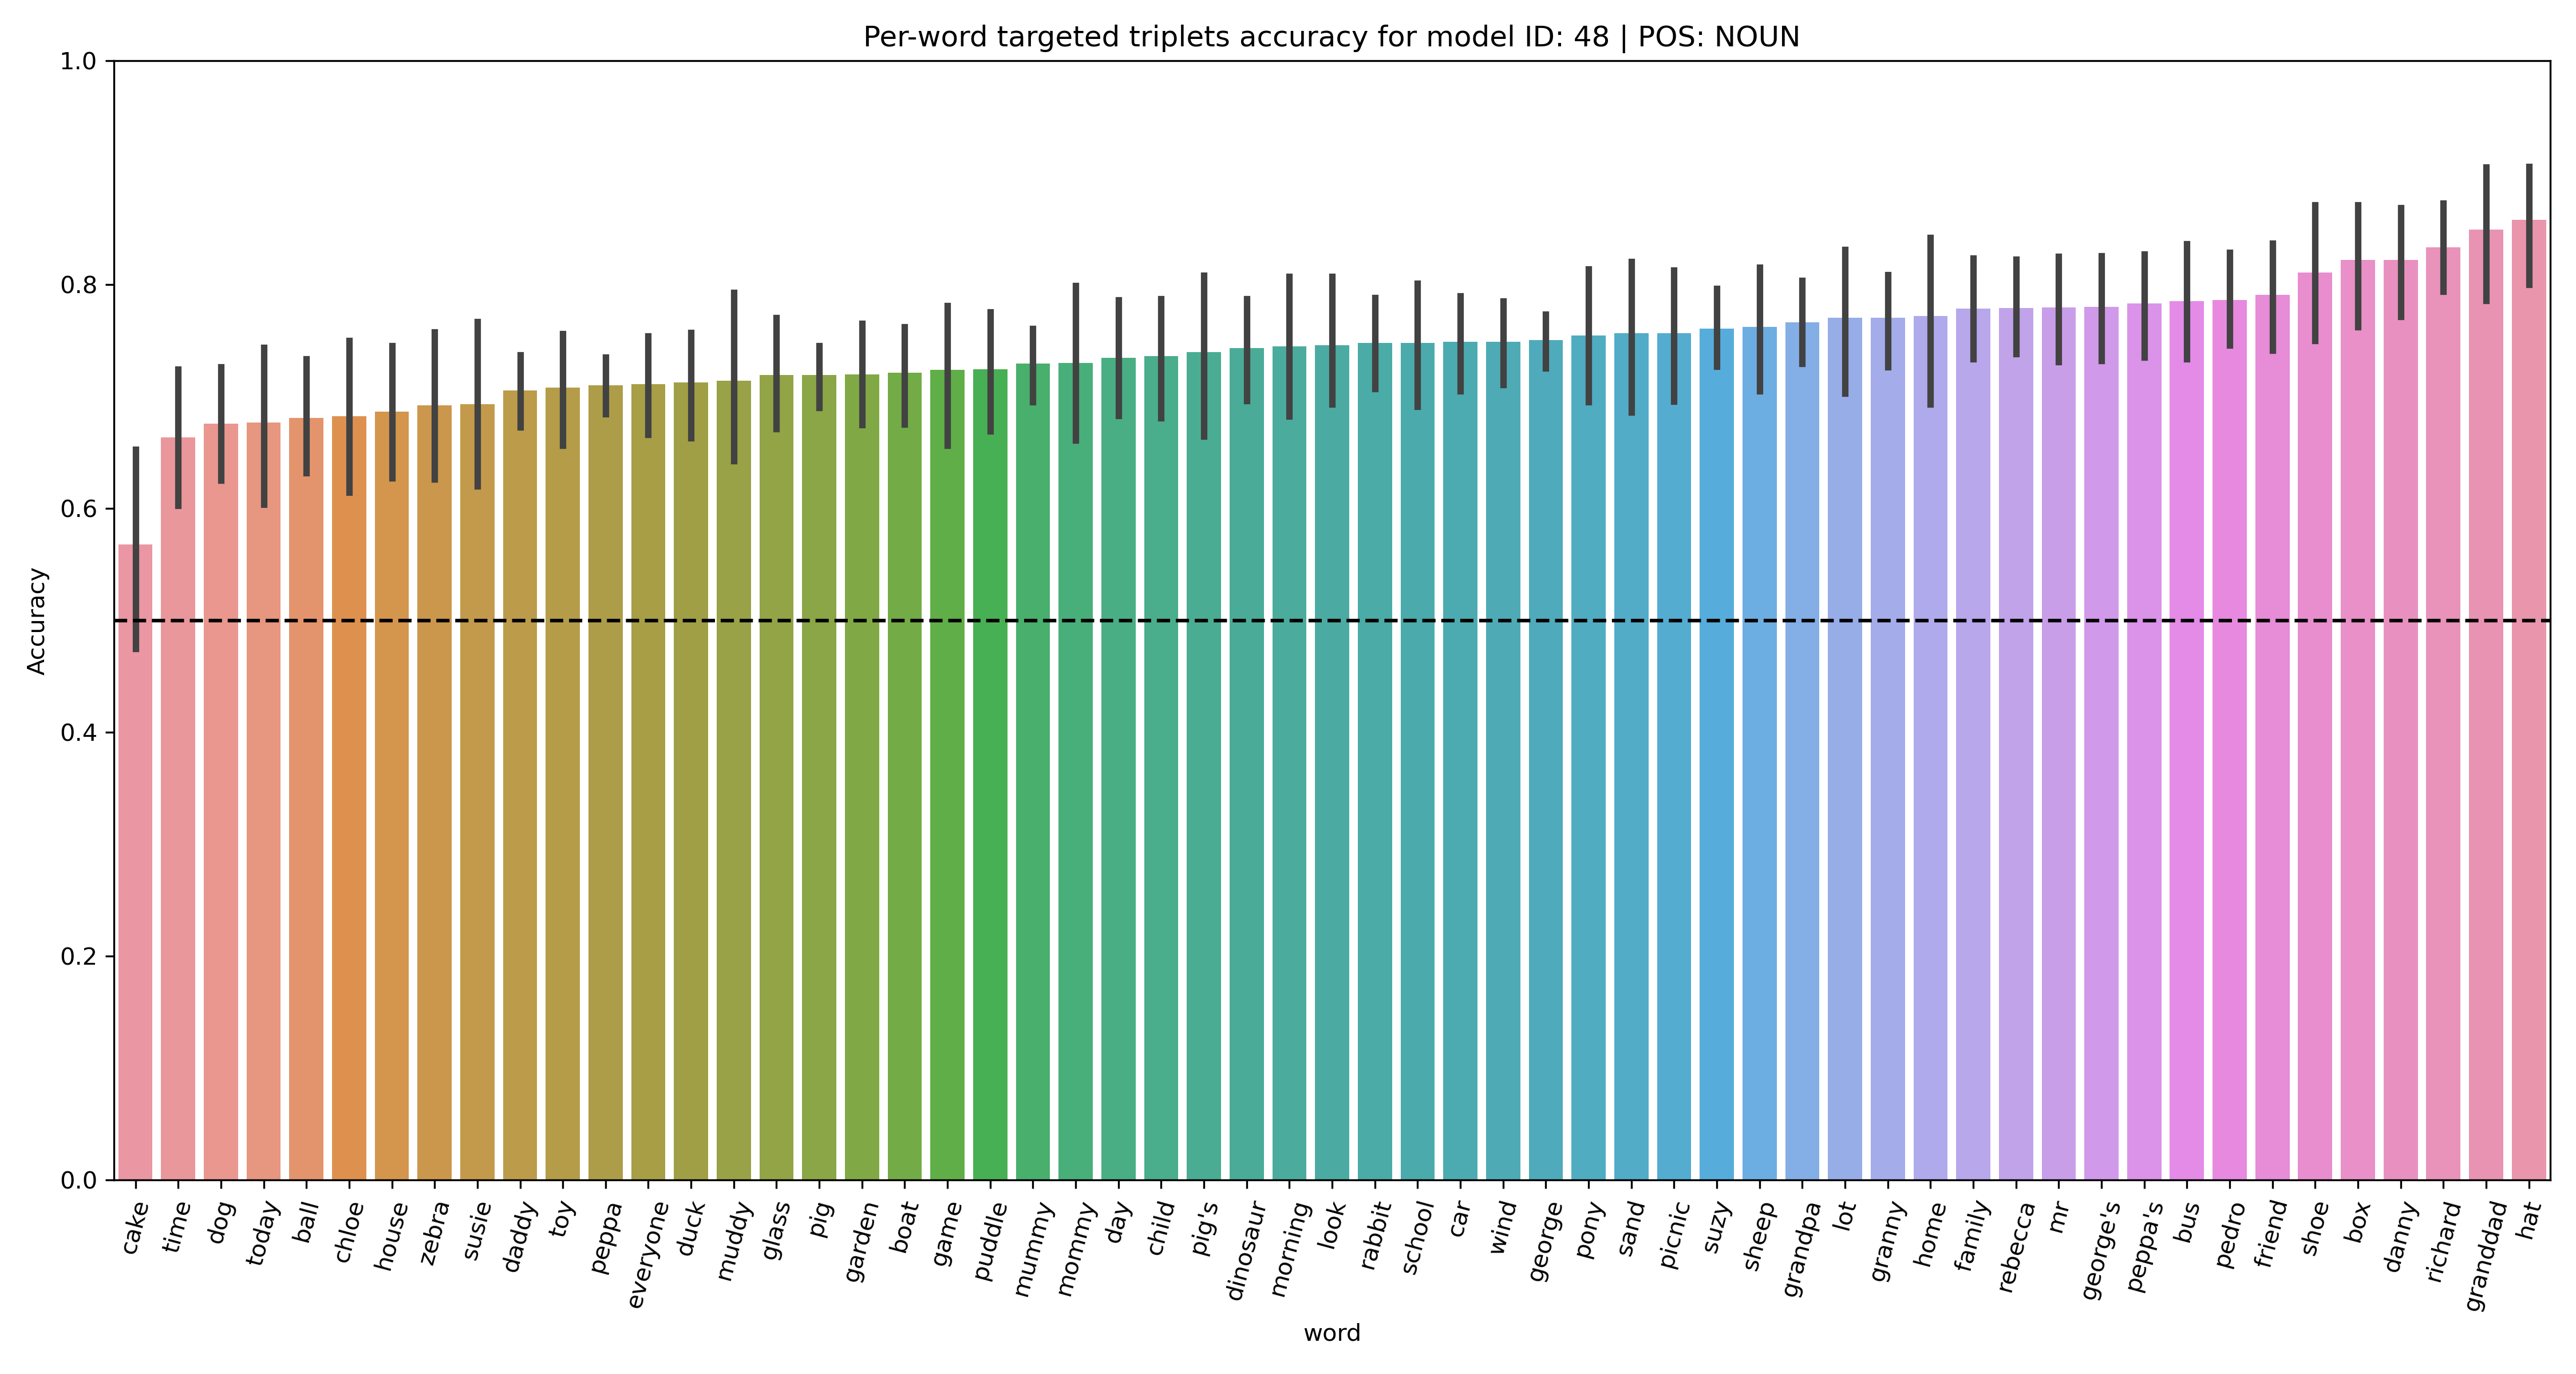
\includegraphics[width=\textwidth]{results_NOUN_word.png}
  \caption{Per-word targeted triplets accuracy for nouns.}
  \label{fig:accuracy_targeted_triplets_nouns}
\end{figure}

\begin{figure}
  \centering
  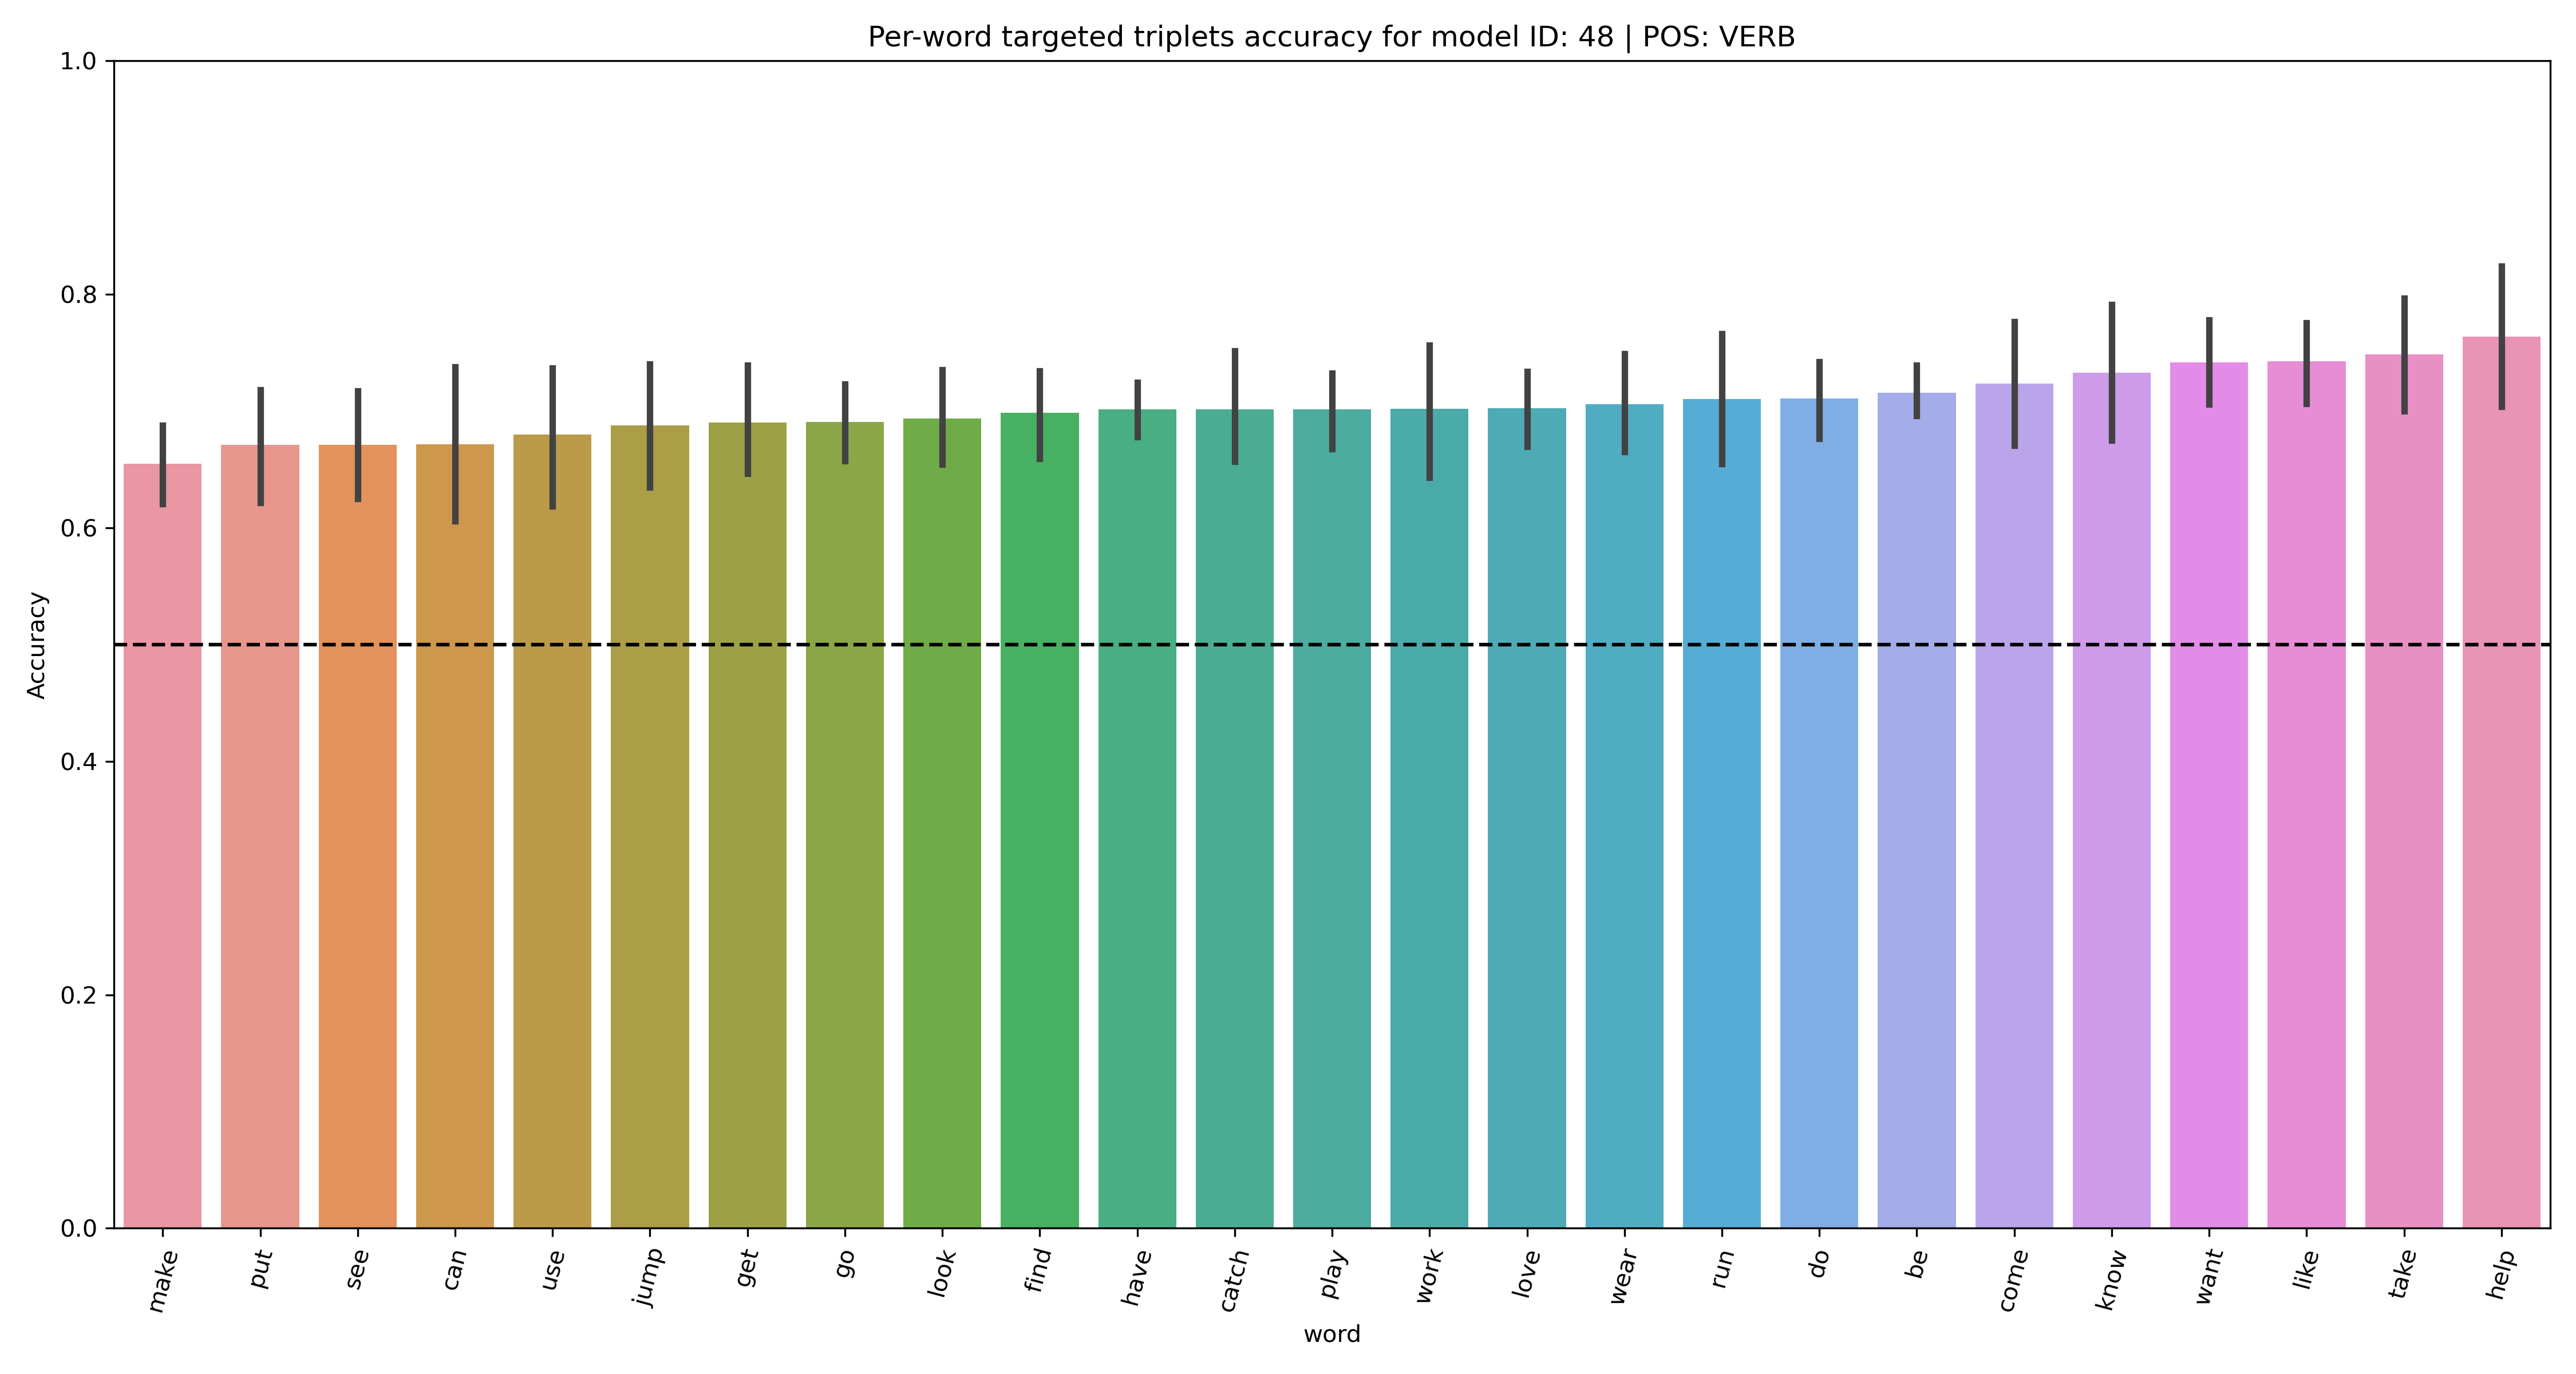
\includegraphics[width=\textwidth]{results_VERB_word.png}
  \caption{Per-word targeted triplets accuracy for verbs.}
  \label{fig:accuracy_targeted_triplets_verbs}
\end{figure}


 
\paragraph{Multiple representational similarity analysis}

For the single-word setting, 
\Cref{tab:dialogvarcor} and \Cref{tab:narrationvarcor} show the raw
correlations between variables in the multiple RSA analysis, while
\Cref{fig:coef_word_dialog} and \Cref{fig:coef_word_narration} show the
standardized regression coefficients, where the target variable is
pairwise representation similarity for the pre-trained-only and the
fully-trained versions of the target model.



\begin{figure}
  \centering
  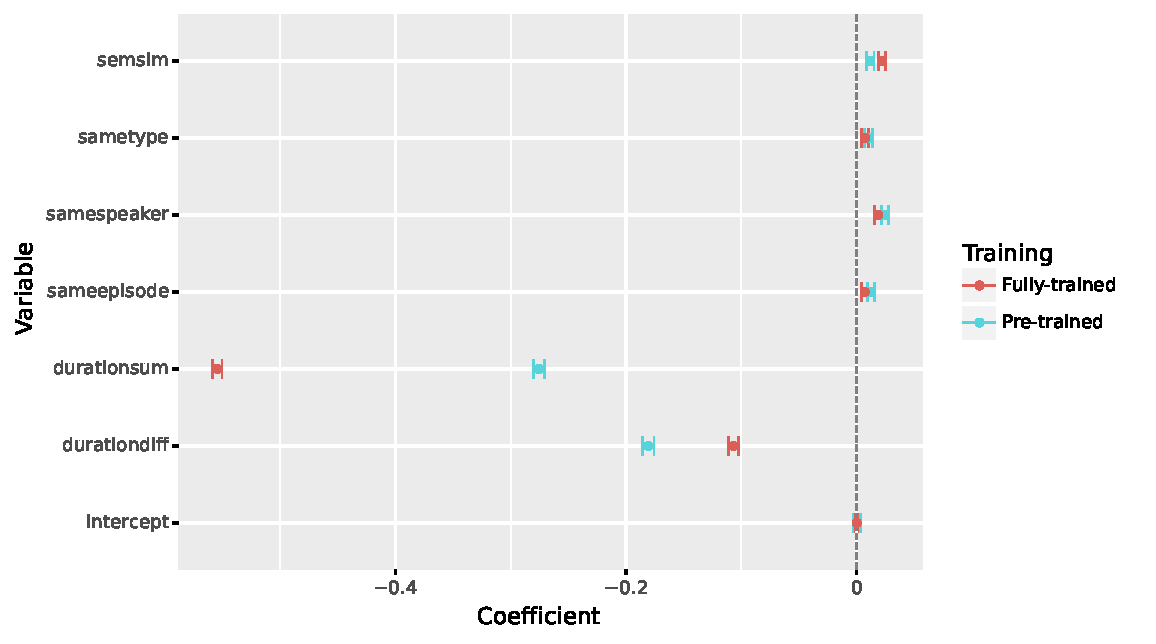
\includegraphics[scale=0.66]{results/grsa_dialog_word_coef.pdf}
  \caption{Association of predictors with trained and untrained
    model-based pairwise similarity scores for single-word utterances
    in the dialog validation data. Coefficients are standardized.}
  \label{fig:coef_word_dialog}
\end{figure}

\begin{figure}
  \centering
  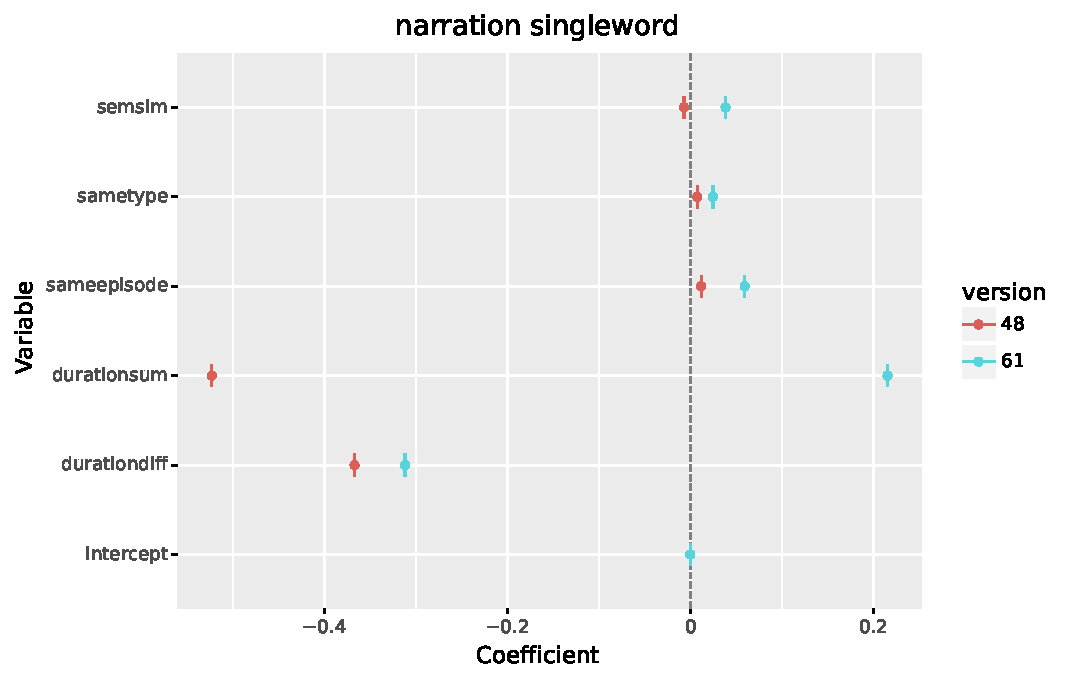
\includegraphics[scale=0.66]{results/grsa_narration_word_coef.pdf}
  \caption{Association of predictors with 
    model-based pairwise similarity scores for single-word utterances
    in the narration validation data. Coefficients are standardized.}
  \label{fig:coef_word_narration}
\end{figure}


For the multi-word setting, \Cref{fig:coef_multiword_dialog} and
\Cref{fig:coef_multiword_narration} show the regression coefficients.
\begin{figure}
  \centering
  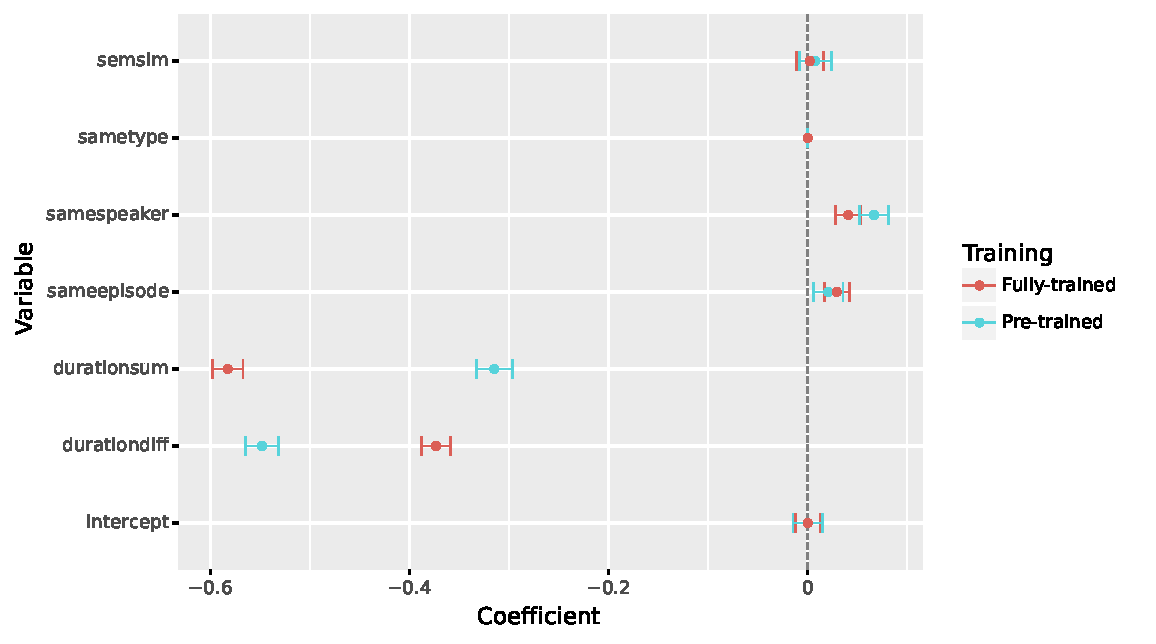
\includegraphics[scale=0.66]{results/grsa_dialog_multiword_coef.pdf}
  \caption{Association of predictors with 
    model-based pairwise similarity scores for multi-word utterances
    in the dialog validation data. Coefficients are standardized.}
  \label{fig:coef_multiword_dialog}
\end{figure}

\begin{figure}
  \centering
  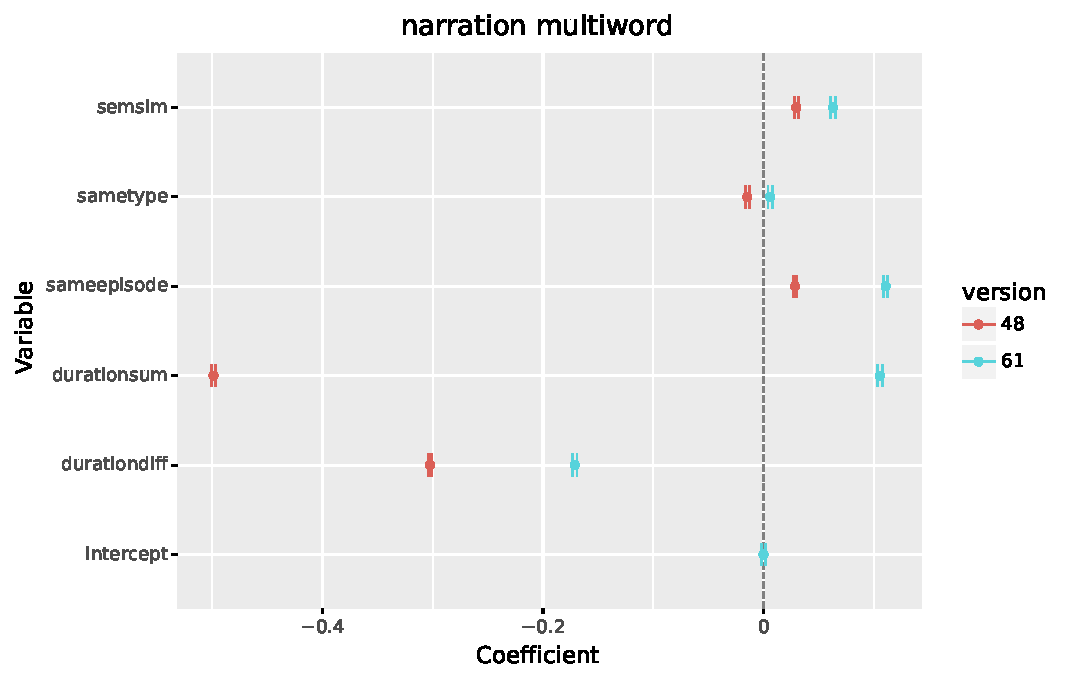
\includegraphics[scale=0.66]{results/grsa_narration_multiword_coef.pdf}
  \caption{Association of predictors with 
    model-based pairwise similarity scores for multi-word utterances
    in the narration validation data. Coefficients are standardized.}
  \label{fig:coef_multiword_narration}
\end{figure}


\todo{Update discussion of results}

%For both data subsets (dialog and narration), the highest magnitude
%predictors are {\tt durationdiff}, {\tt durationsum} and {\tt semsim}. The effect of
%the {\tt samespeaker} predictor for the dialog data is close to zero.
%These effect are there already for the pre-trained-only
%representations, but are strengthened for the fully-trained target
%model.  This results indicate that the model learns some aspects of
%word-level semantics as captured by GloVe word vectors, and that
%speaker identity does not appear to be a substantial impact on
%utterance embeddings.

The strength of the association between effects of utterance
duration {\tt durationdiff}, {\tt durationsum} and pairwise similarities apparent in this
data was suprising and possibly undesirable. We conjecture that is
arises as an effect of the positional encodings in the transformer
layers.

